\documentclass[10pt,journal,compsoc,fleqn]{IEEEtran}
\usepackage{graphicx}
\usepackage{amsmath}
\usepackage{amsfonts}
\usepackage{epstopdf}
\usepackage{CJKutf8}
\usepackage{algorithm, algorithmic}
\newtheorem{thm}{{Theorem}}[section]
\newtheorem{defn}{Definition}[section]
\newtheorem{lem}{Lemma}[section]
\newtheorem{rmk}{Remark}[section]
\newenvironment{proof}{\noindent {\bf Proof: }}\\


\hyphenation{op-tical net-works semi-conduc-tor}


\begin{document}
\begin{CJK}{UTF8}{song}
\title{Test}
\author{龙威帆}
\maketitle


\section{测试计划}
Pyqt自带的文档没有函数介绍,只写了函数名,连函数用来干嘛的都没写,看不懂。所以采用人力测试。

\section{测试用例}
1.不输入题目数,点击commit按钮;\\
2.分别输入字符串,负数,大于1000的整数,0,1000,点击commit按钮;\\
3.初始界面点击各个按钮,测试是否存在题目未出现就能点击的状况;\\
4.输入一个正常大于5且非5的倍数的整数,点击commit按钮,查看功能是否完成;\\
5.在第一页的时候,点击 last page按钮,查看是否造成数组越界;\\
6.点击next page按钮,查看功能是否完成;\\
7.在最后一页的时候,点击 next page按钮,查看是否造成数组越界;\\
8.随便输入几个答案(字符串,负数等),点击 check results按钮,查看功能是否完成;\\
9.点击view answers按钮,查看功能是否完成。
\section{测试报告}
用例1,结果如下图(Fig. \ref{Test_1}),弹出警告窗口。
\begin{figure}[H]
  \centering
  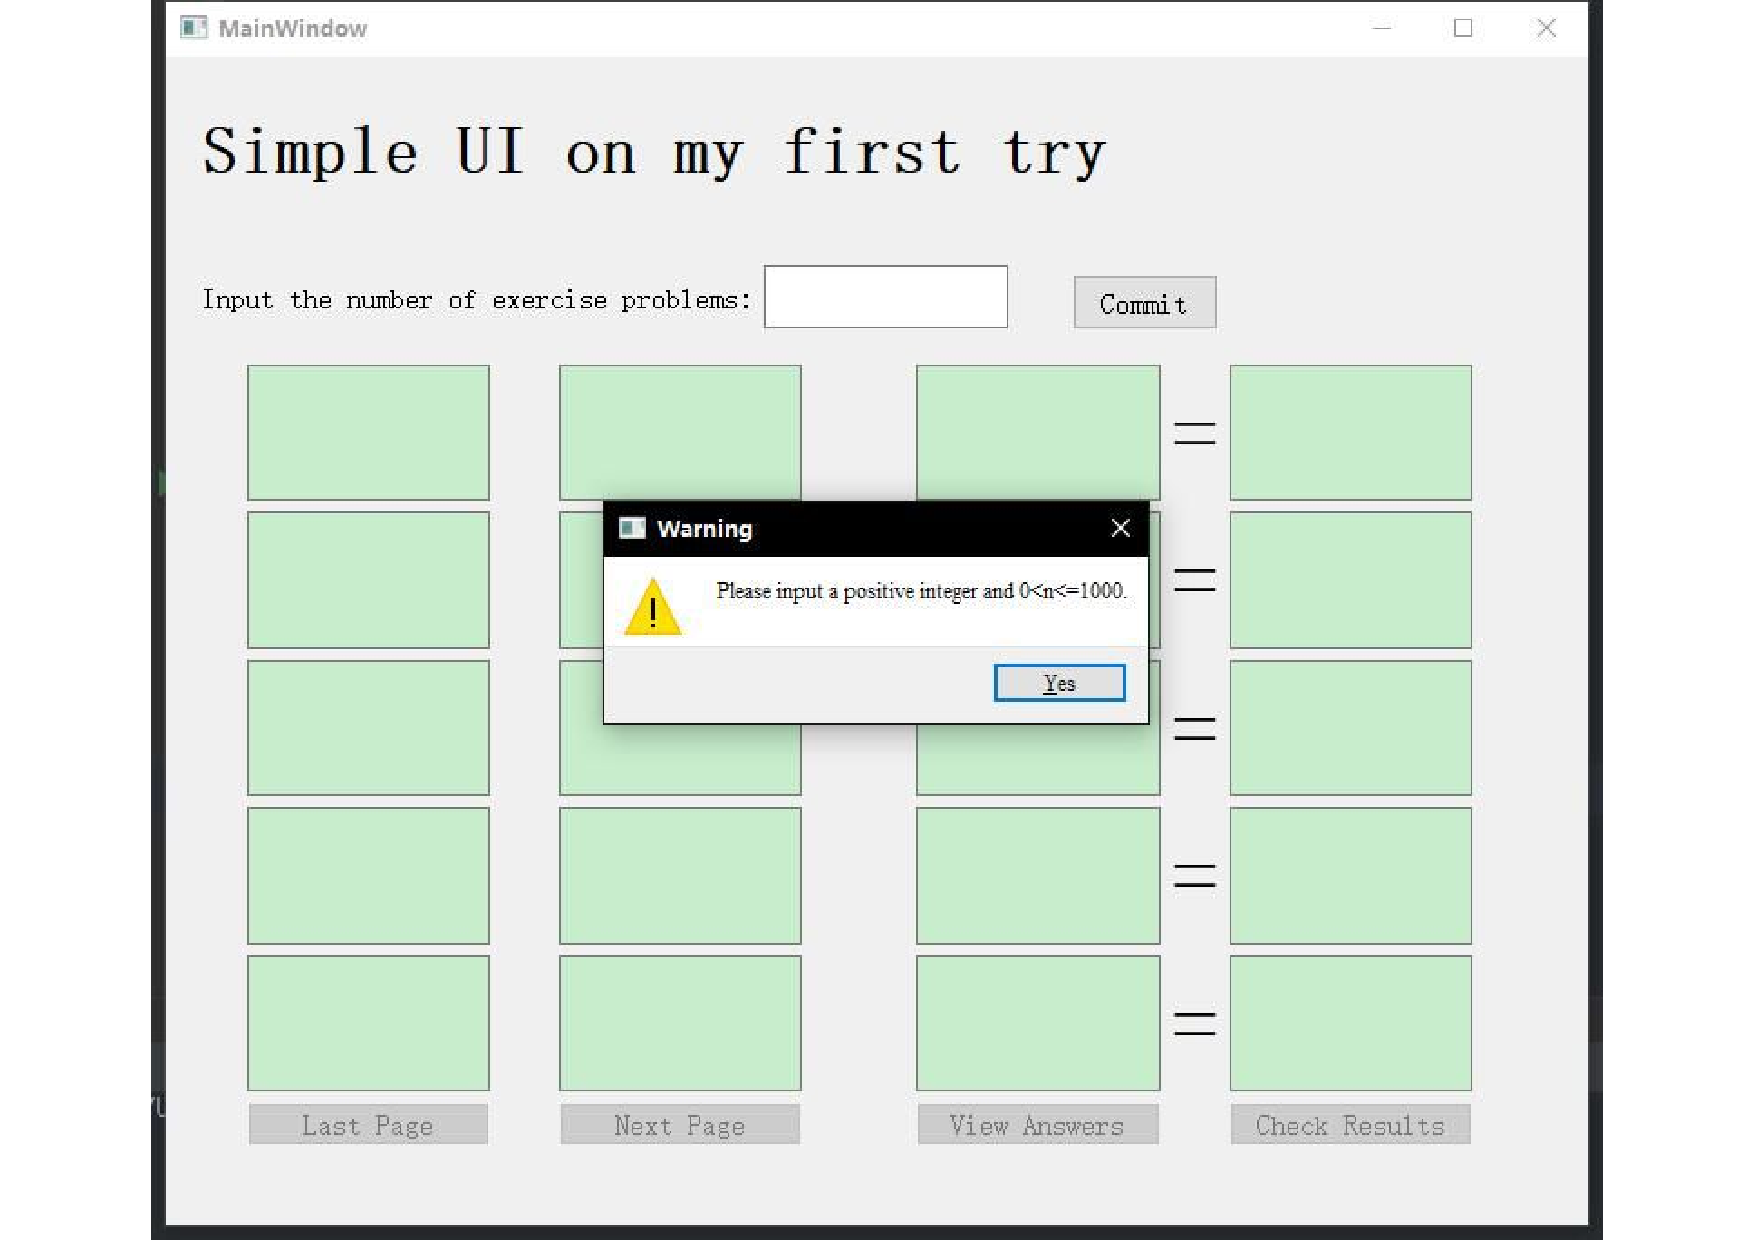
\includegraphics[width=2.5in]{./figures/1.pdf}
  \caption{Test 1}
  \label{Test_1}
\end{figure}
用例2,结果都如下图(Fig. \ref{Test_2}),弹出警告窗口。
\begin{figure}[H]
  \centering
  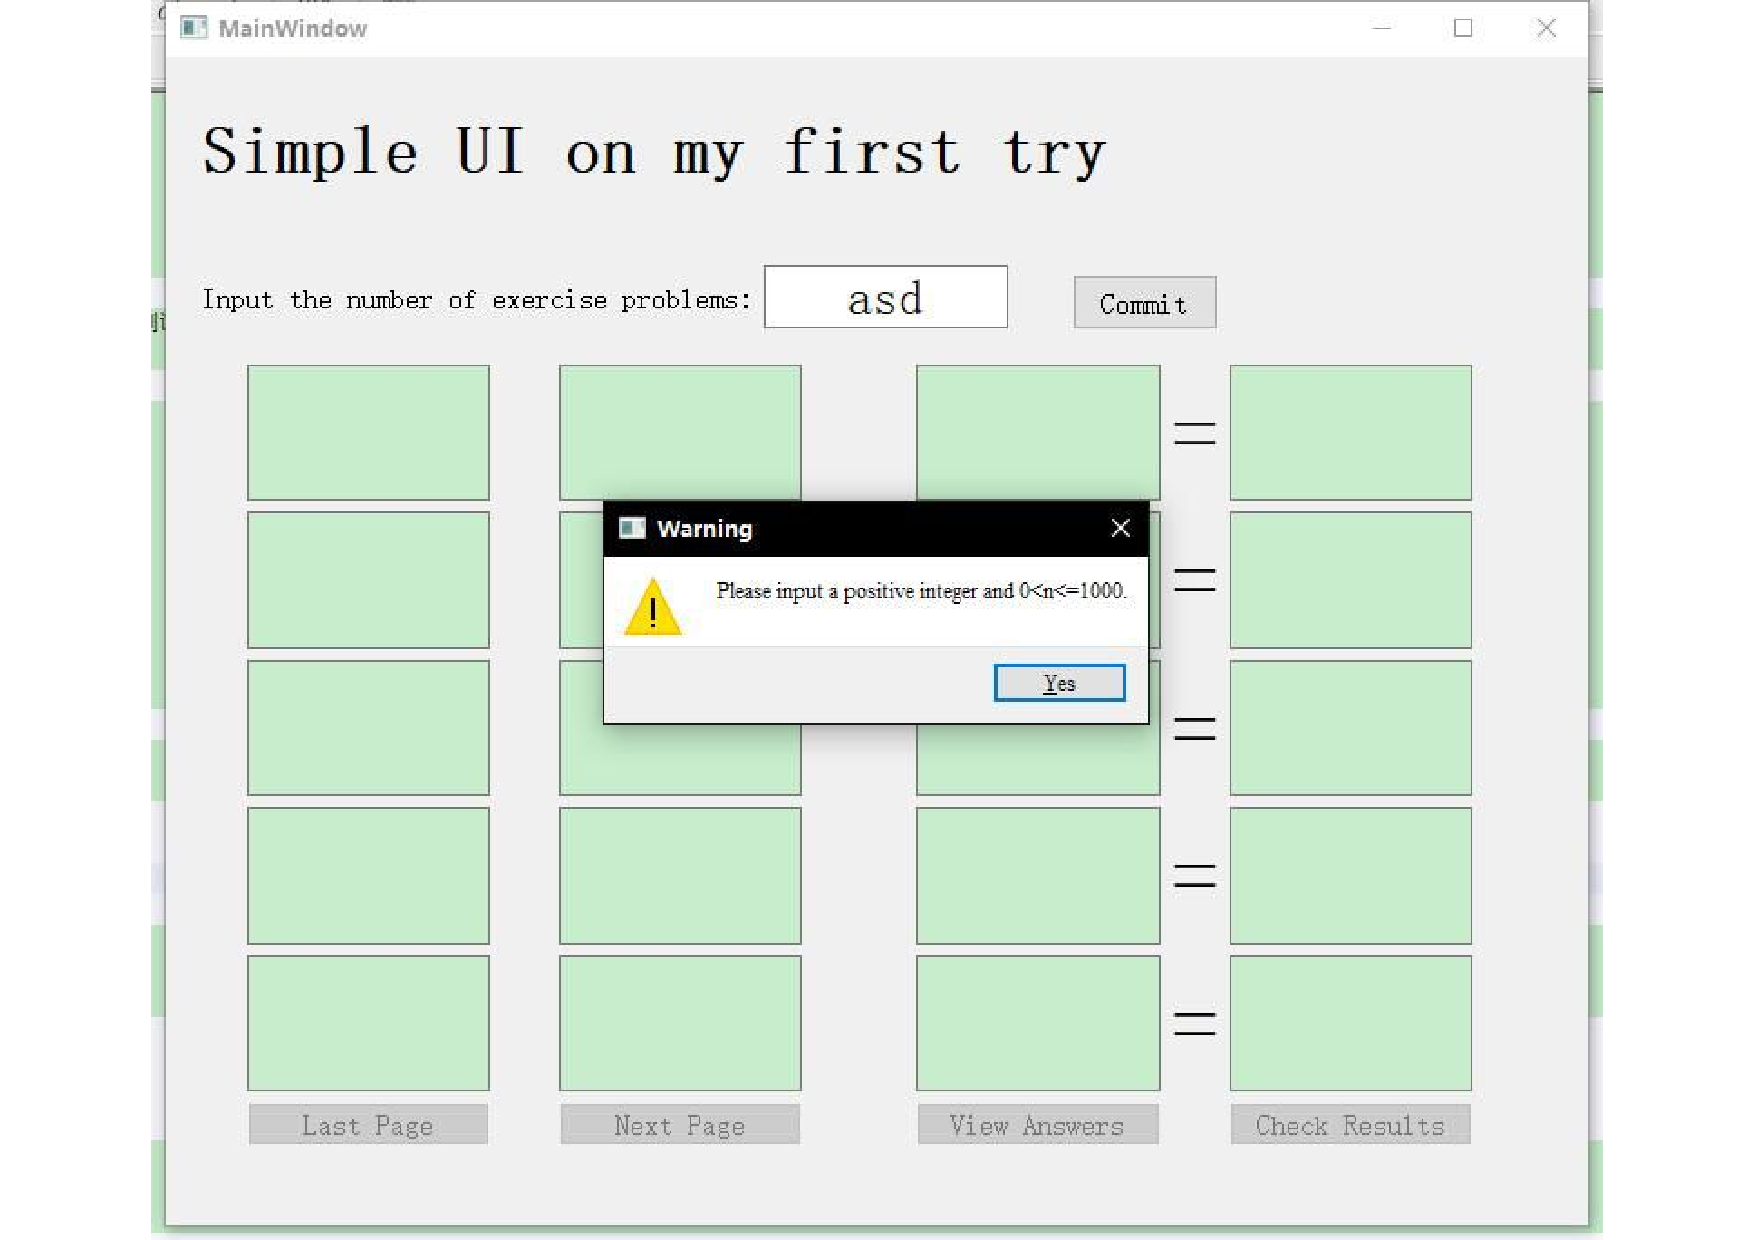
\includegraphics[width=2.5in]{./figures/2.pdf}
  \caption{Test 2}
  \label{Test_2}
\end{figure}
用例3,结果如下图(Fig. \ref{Test_3}), 除Commmit按钮外,均不可点击。
\begin{figure}[H]
  \centering
  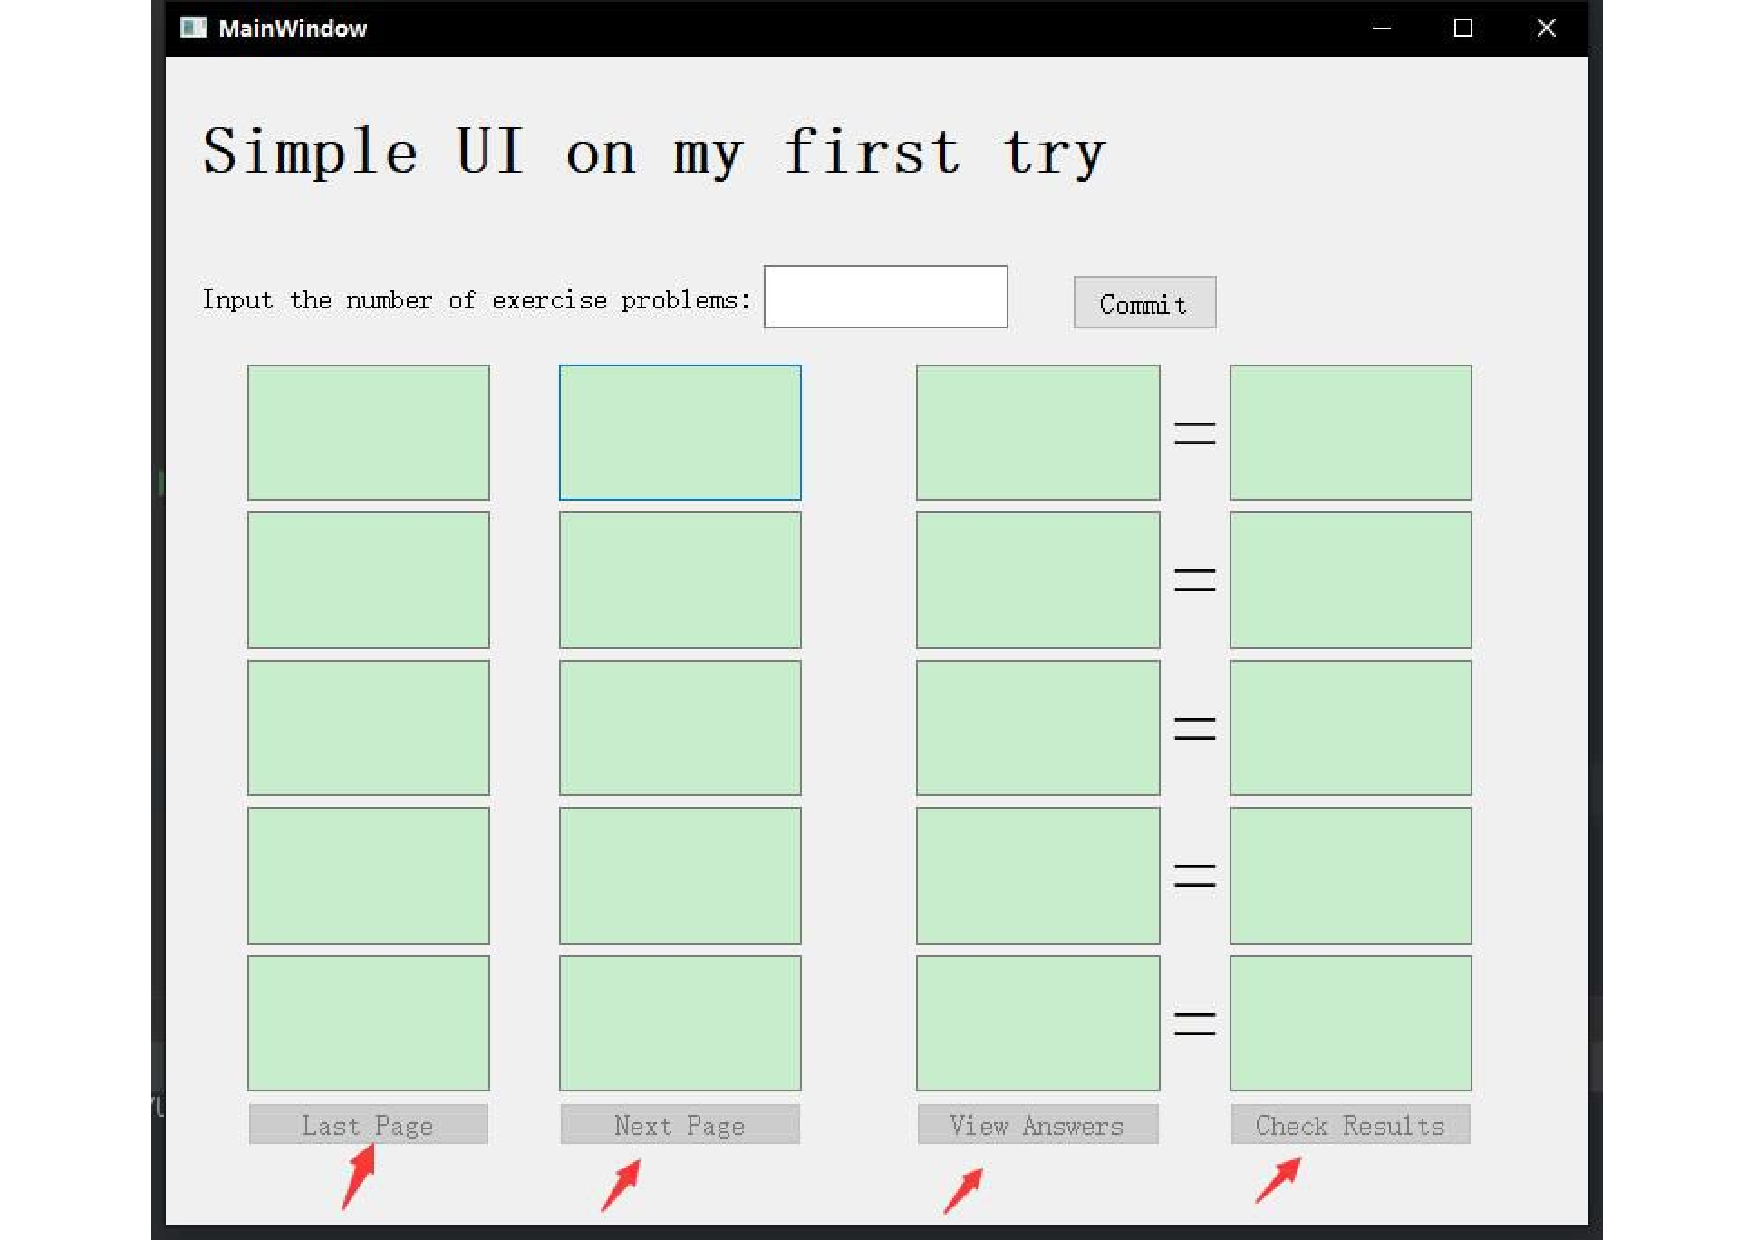
\includegraphics[width=2.5in]{./figures/4.pdf}
  \caption{Test 3}
  \label{Test_3}
\end{figure}
用例4,结果如下图(Fig. \ref{Test_4}),功能实现。
\begin{figure}[H]
  \centering
  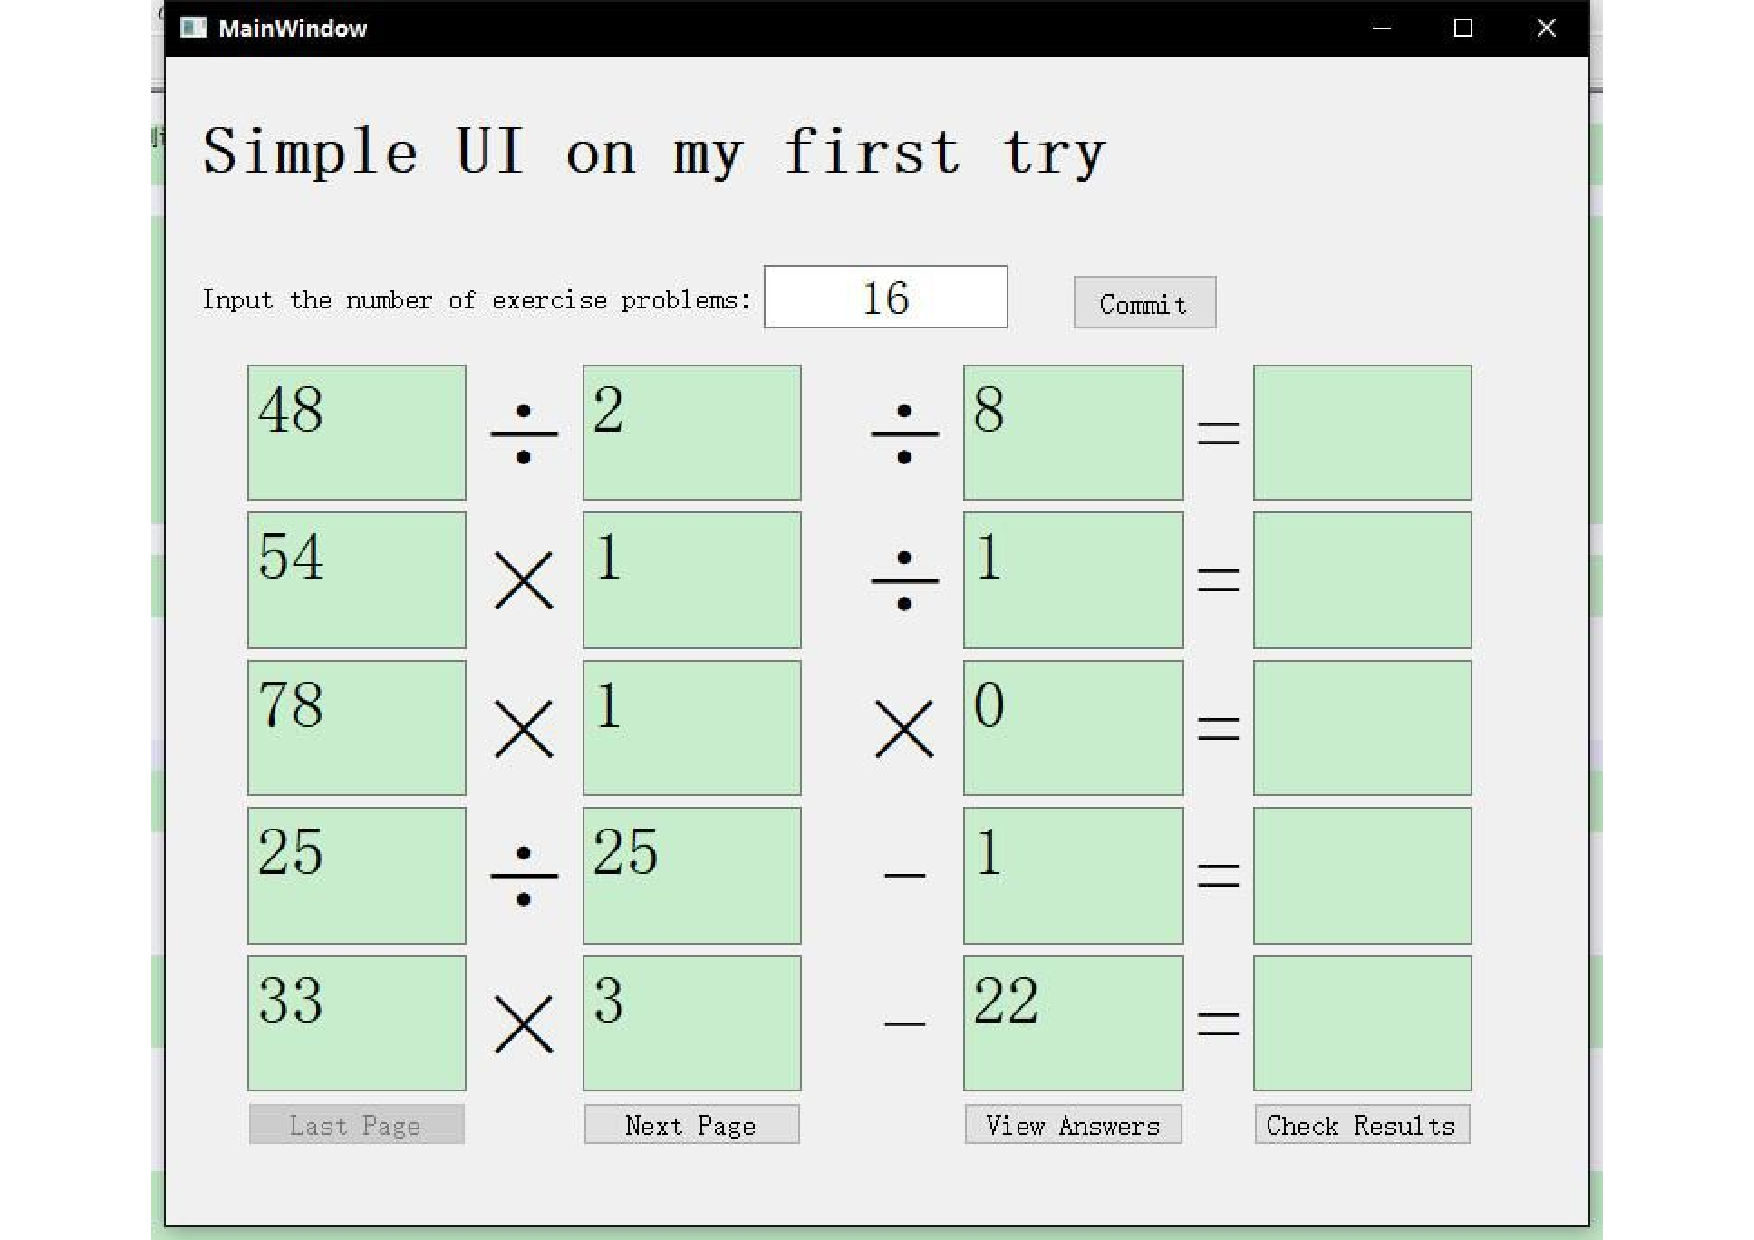
\includegraphics[width=2.5in]{./figures/3.pdf}
  \caption{Test 4}
  \label{Test_4}
\end{figure}
用例5,结果如下图(Fig. \ref{Test_5}),不可点击。
\begin{figure}[H]
  \centering
  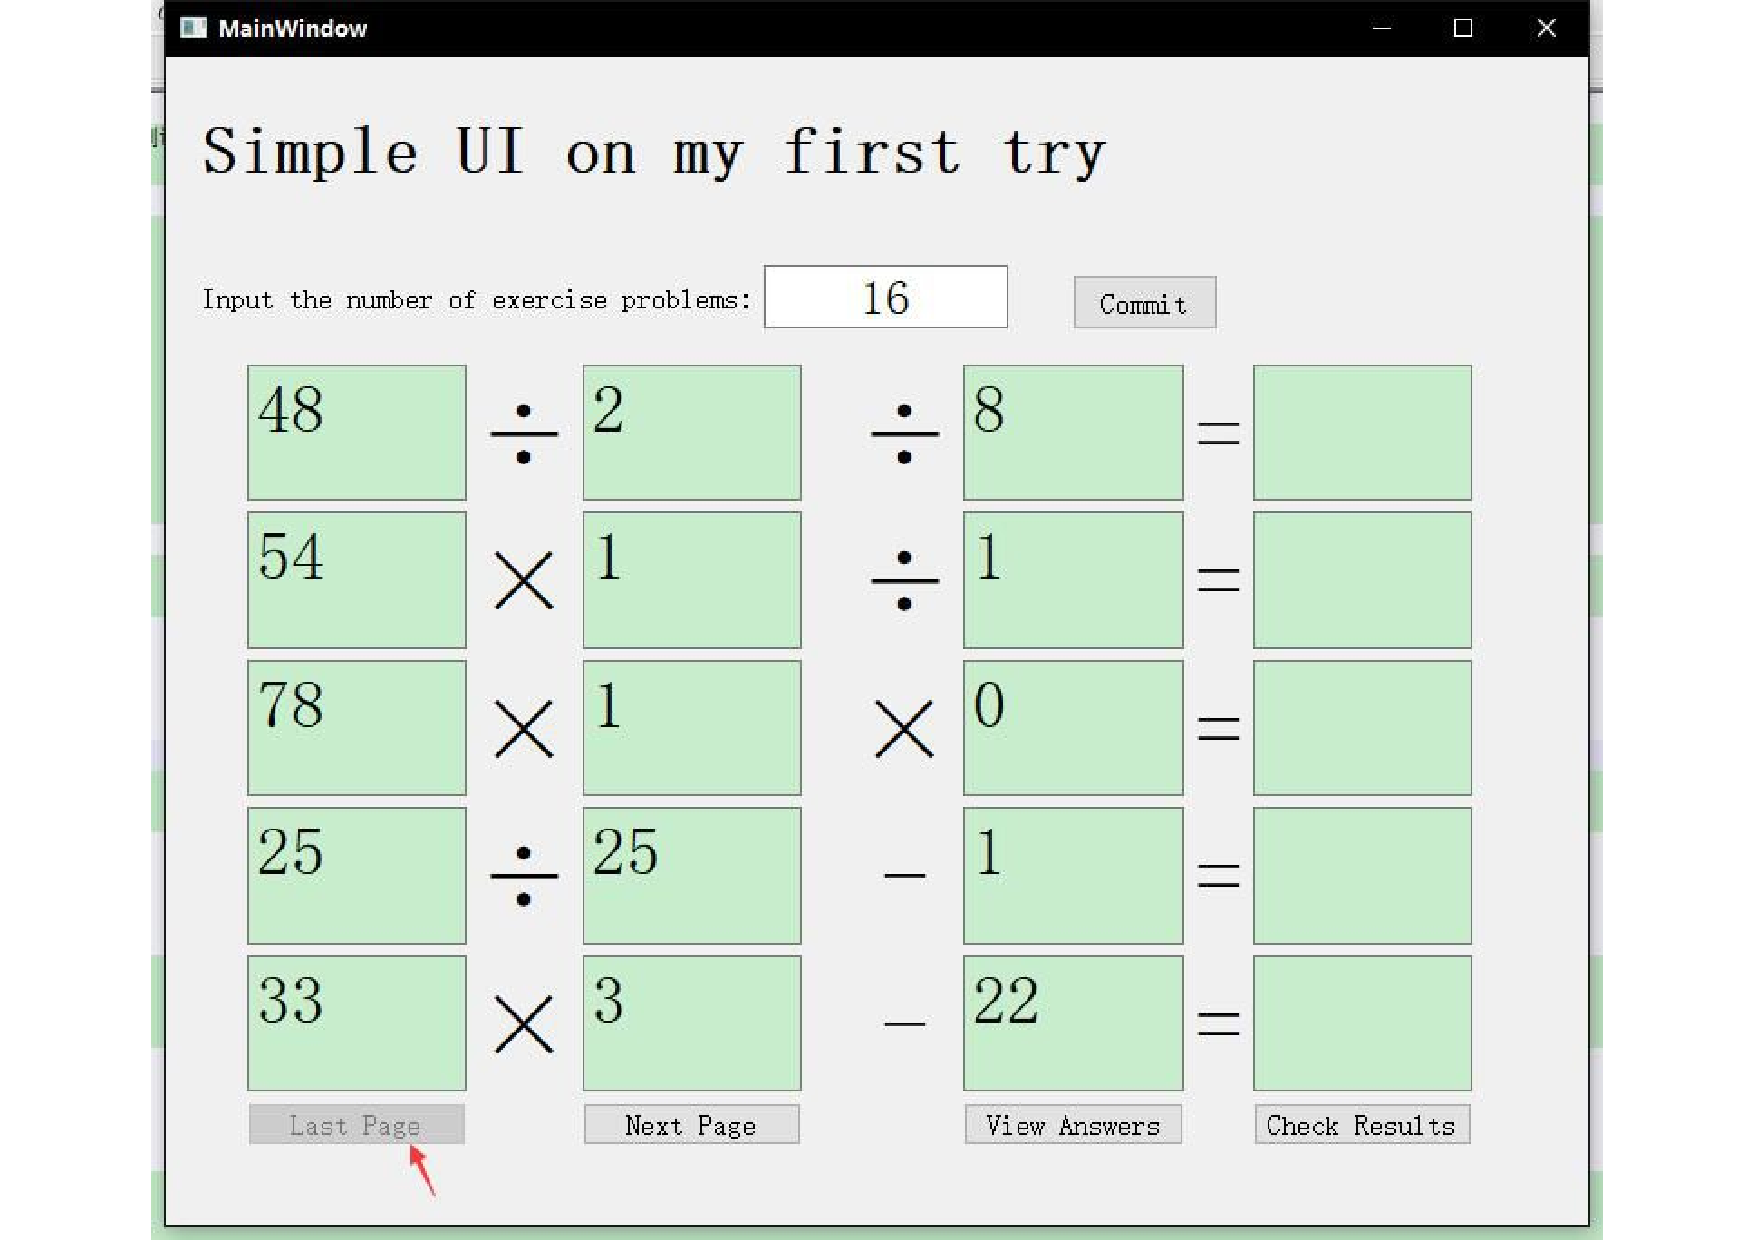
\includegraphics[width=2.5in]{./figures/5.pdf}
  \caption{Test 5}
  \label{Test_5}
\end{figure}
用例6,结果如下图(Fig. \ref{Test_6}),功能实现。
\begin{figure}[H]
  \centering
  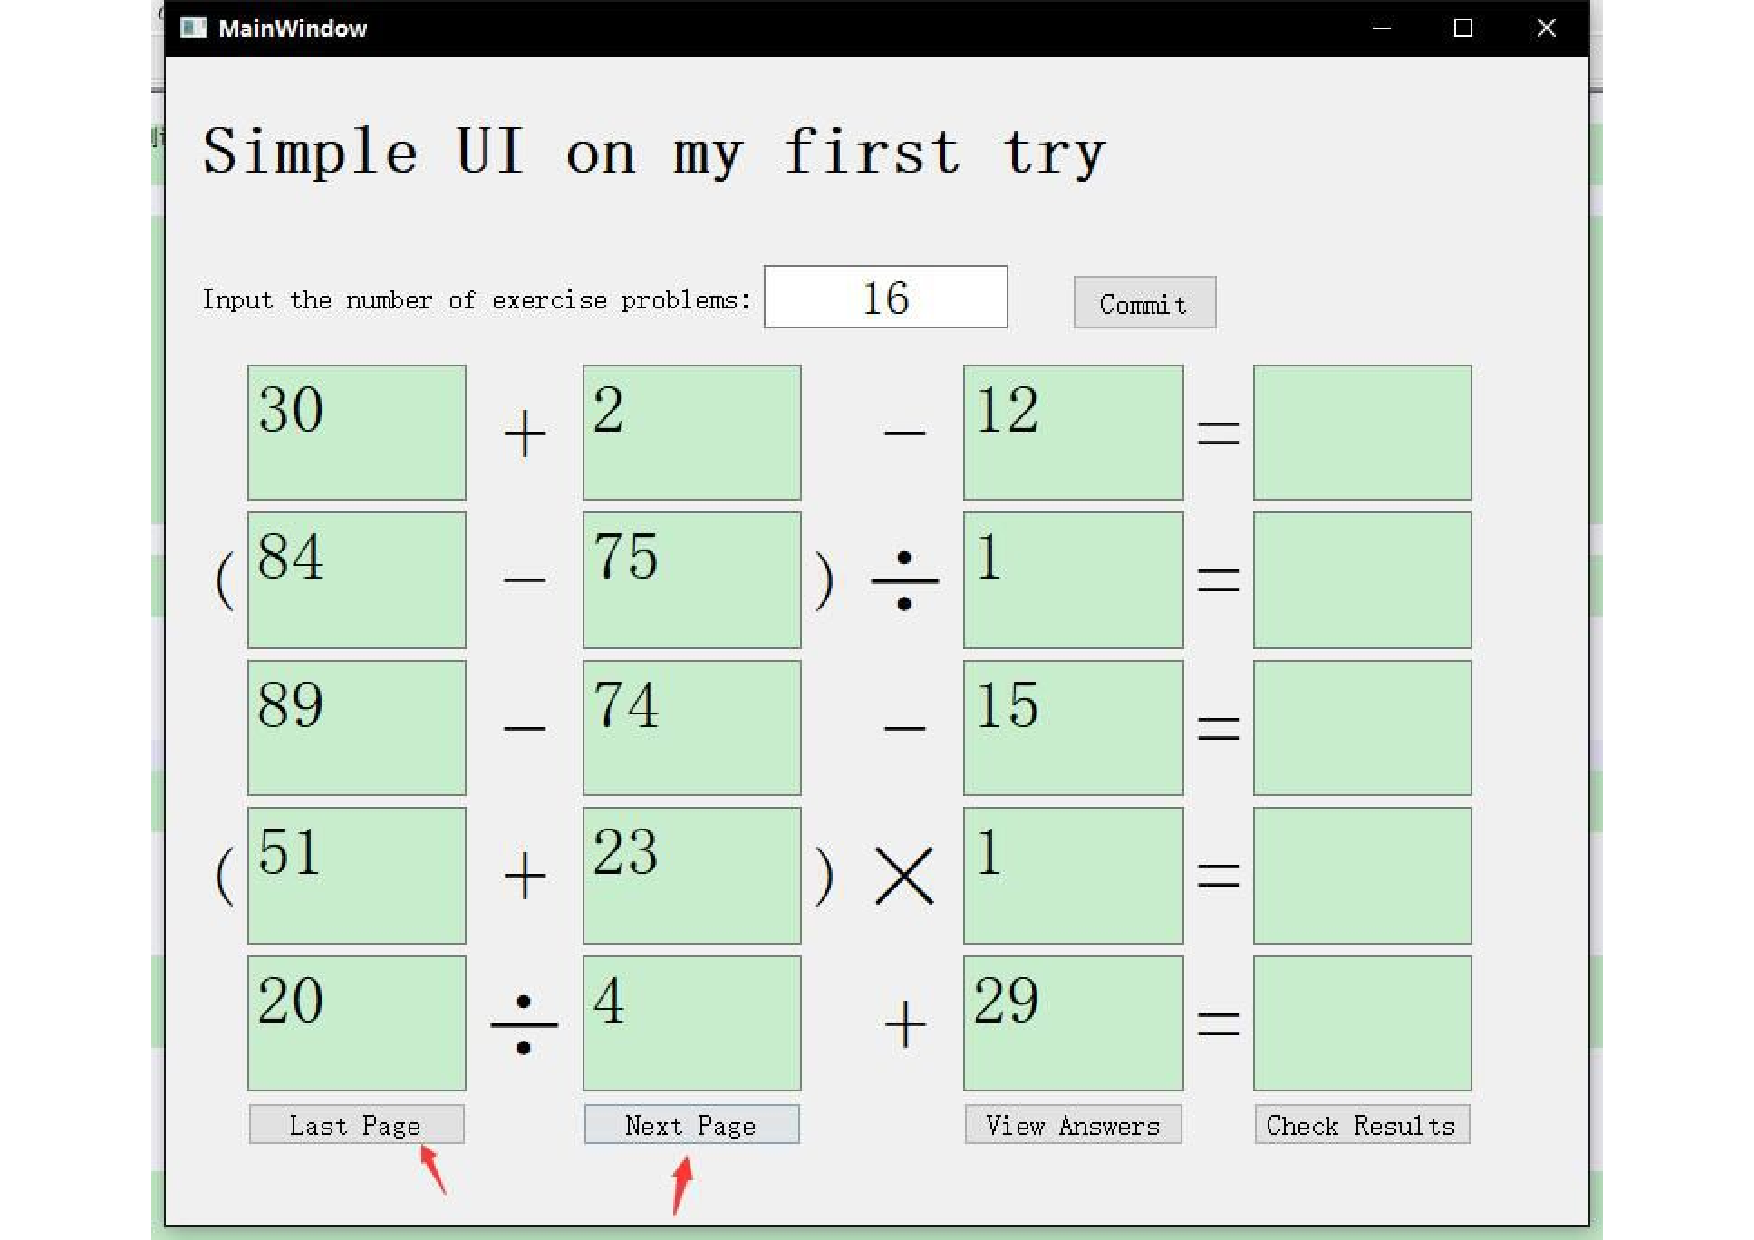
\includegraphics[width=2.5in]{./figures/6.pdf}
  \caption{Test 6}
  \label{Test_6}
\end{figure}
用例7,结果如下图(Fig. \ref{Test_7}),不可点击,不会越界。
\begin{figure}[H]
  \centering
  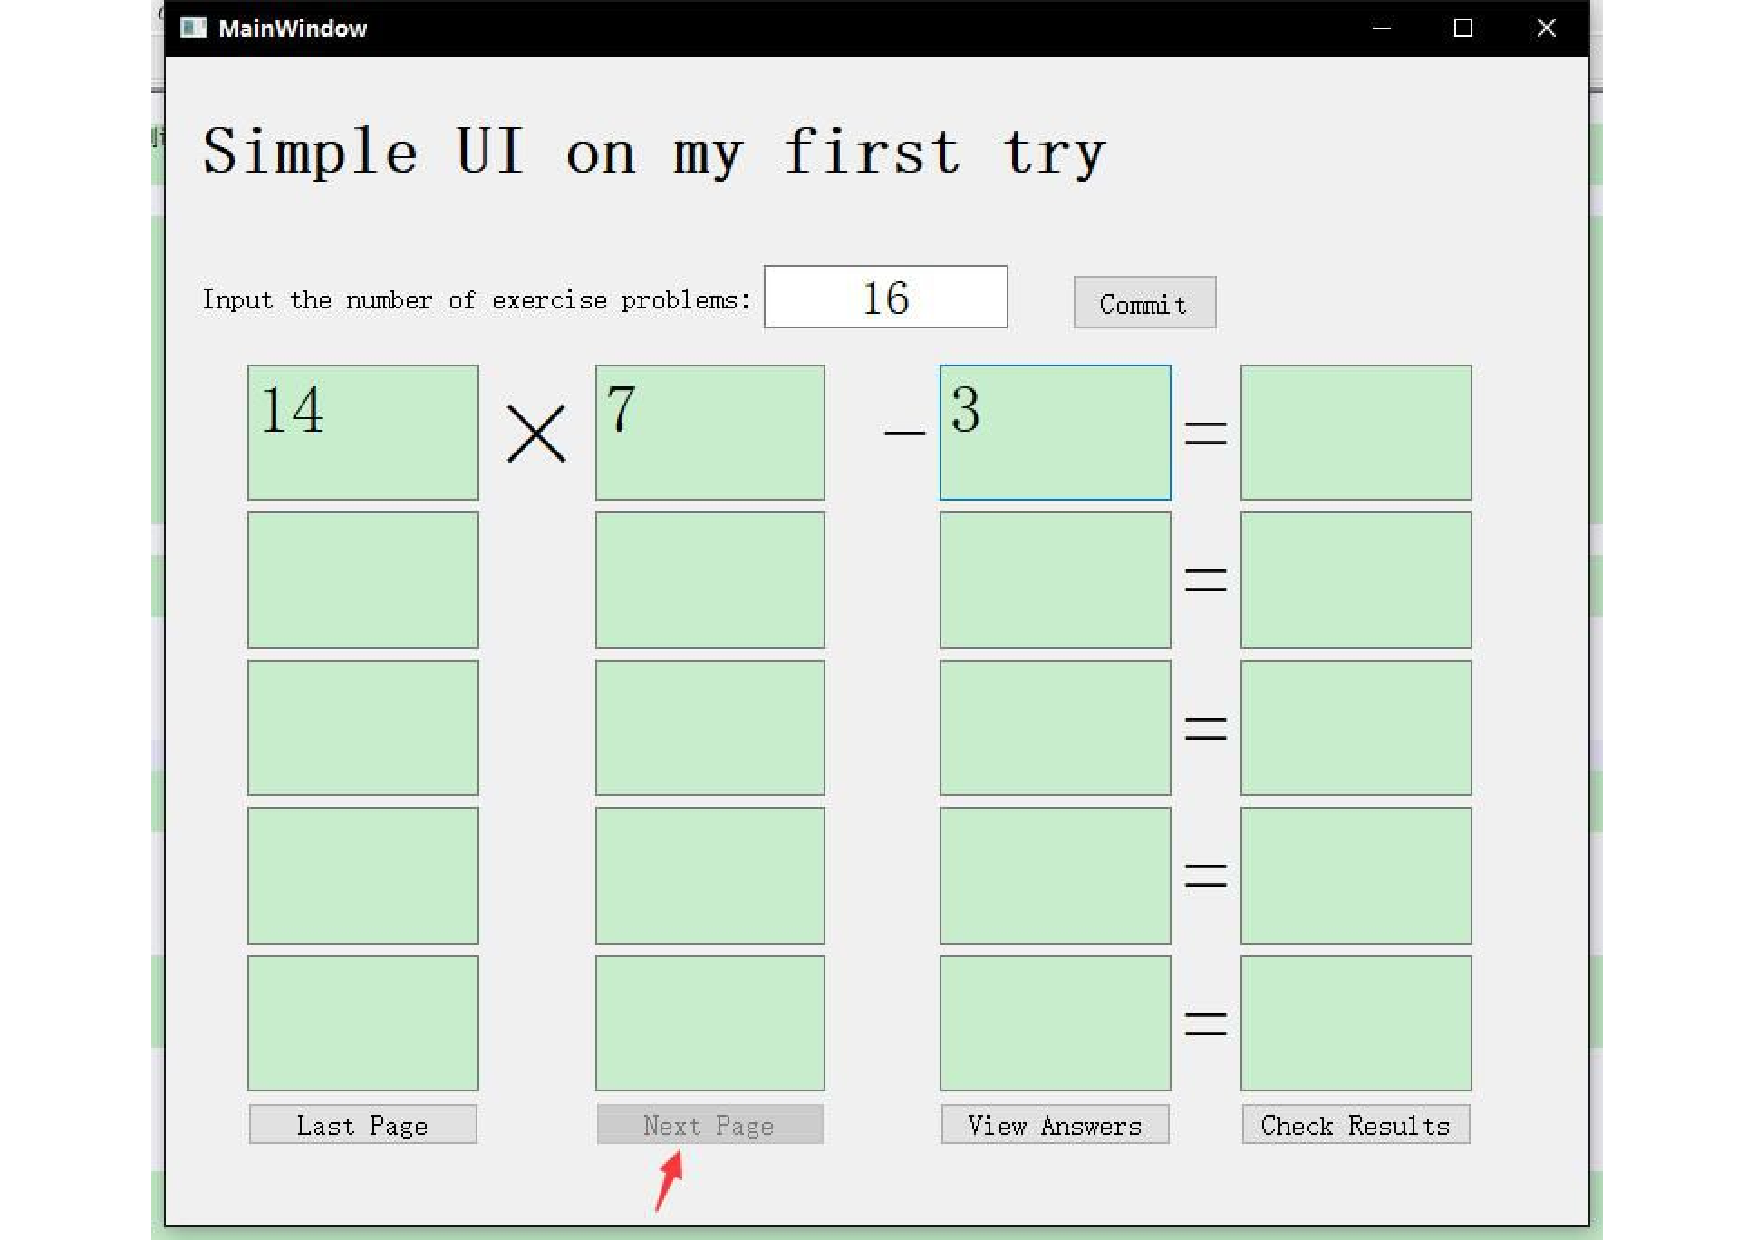
\includegraphics[width=2.5in]{./figures/7.pdf}
  \caption{Test 7}
  \label{Test_7}
\end{figure}
用例8,结果如下图(Fig. \ref{Test_8}),功能实现。
\begin{figure}[H]
  \centering
  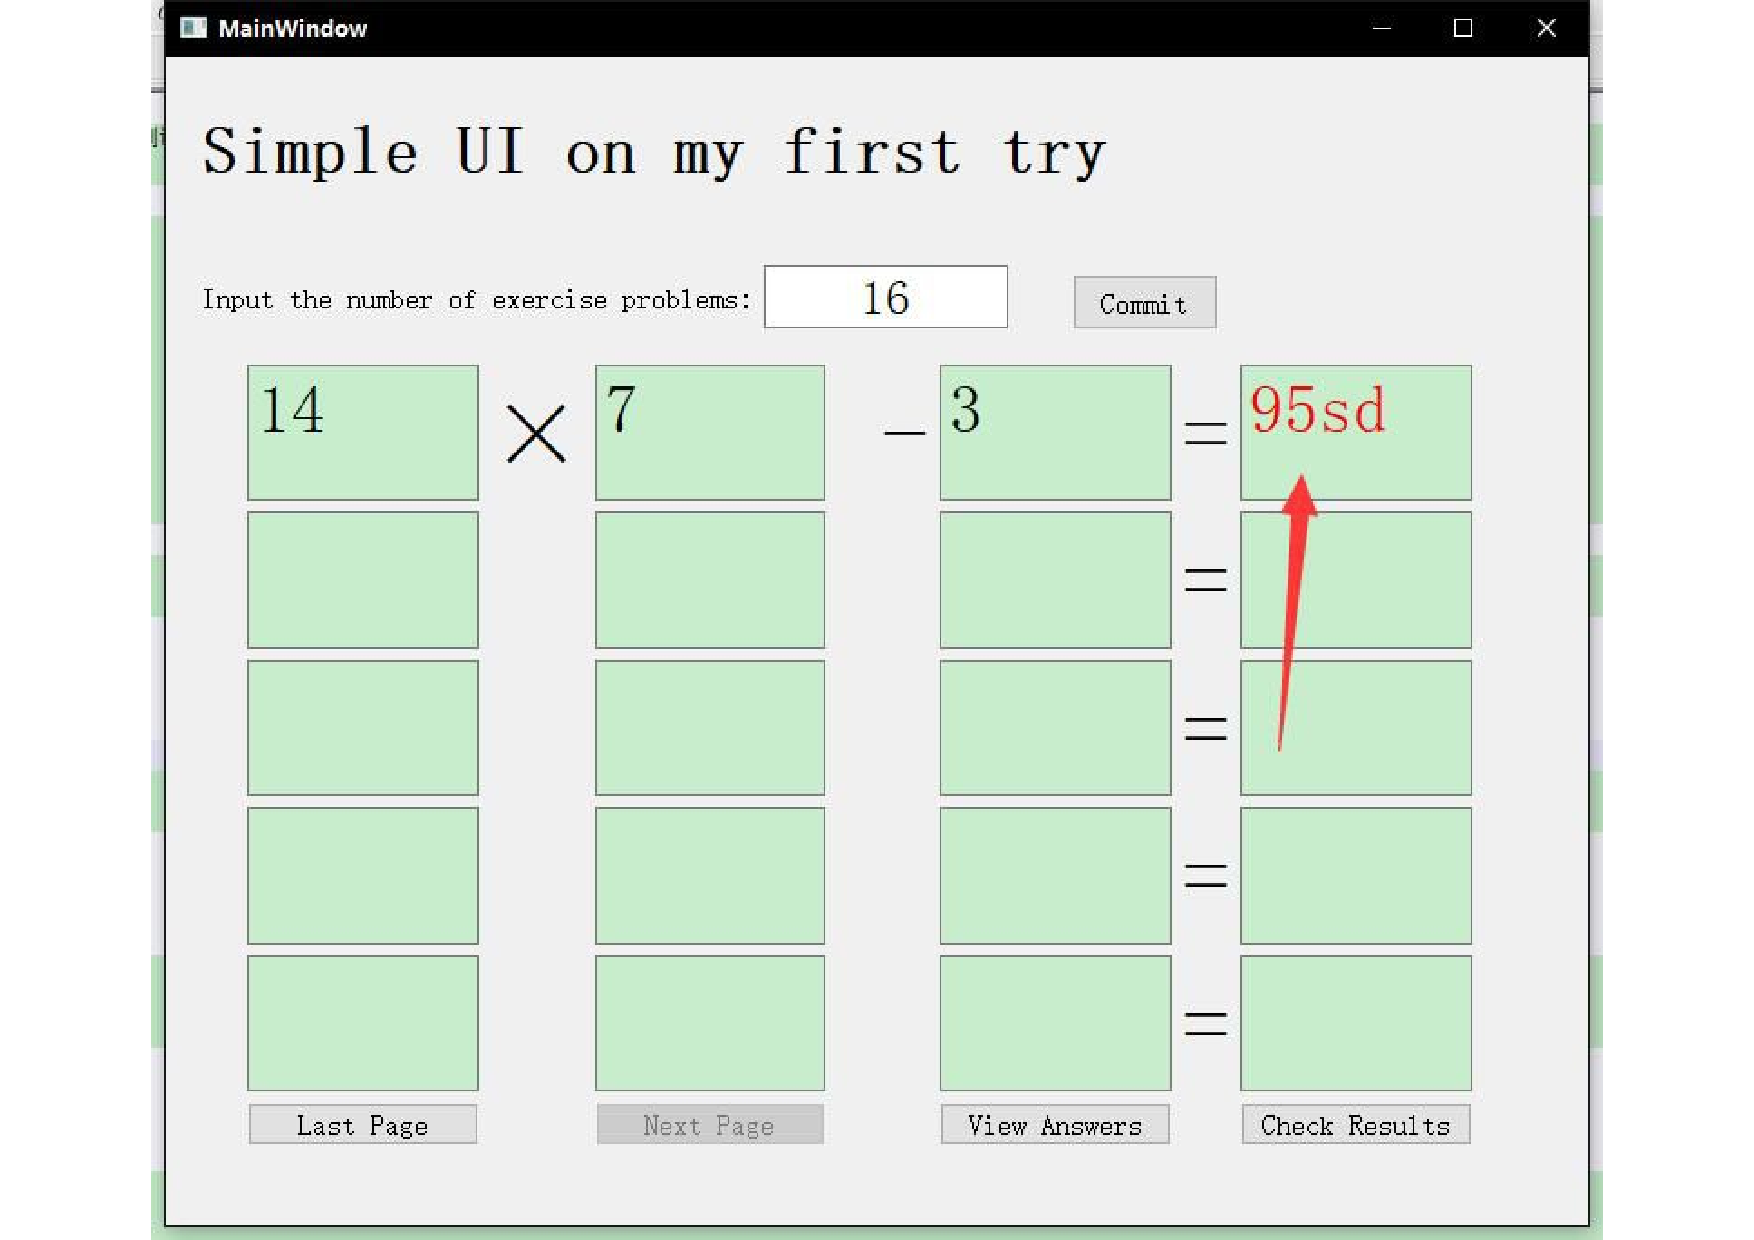
\includegraphics[width=2.5in]{./figures/8.pdf}
  \caption{Test 8}
  \label{Test_8}
\end{figure}
用例9,结果如下图(Fig. \ref{Test_9}),功能实现。
\begin{figure}[H]
  \centering
  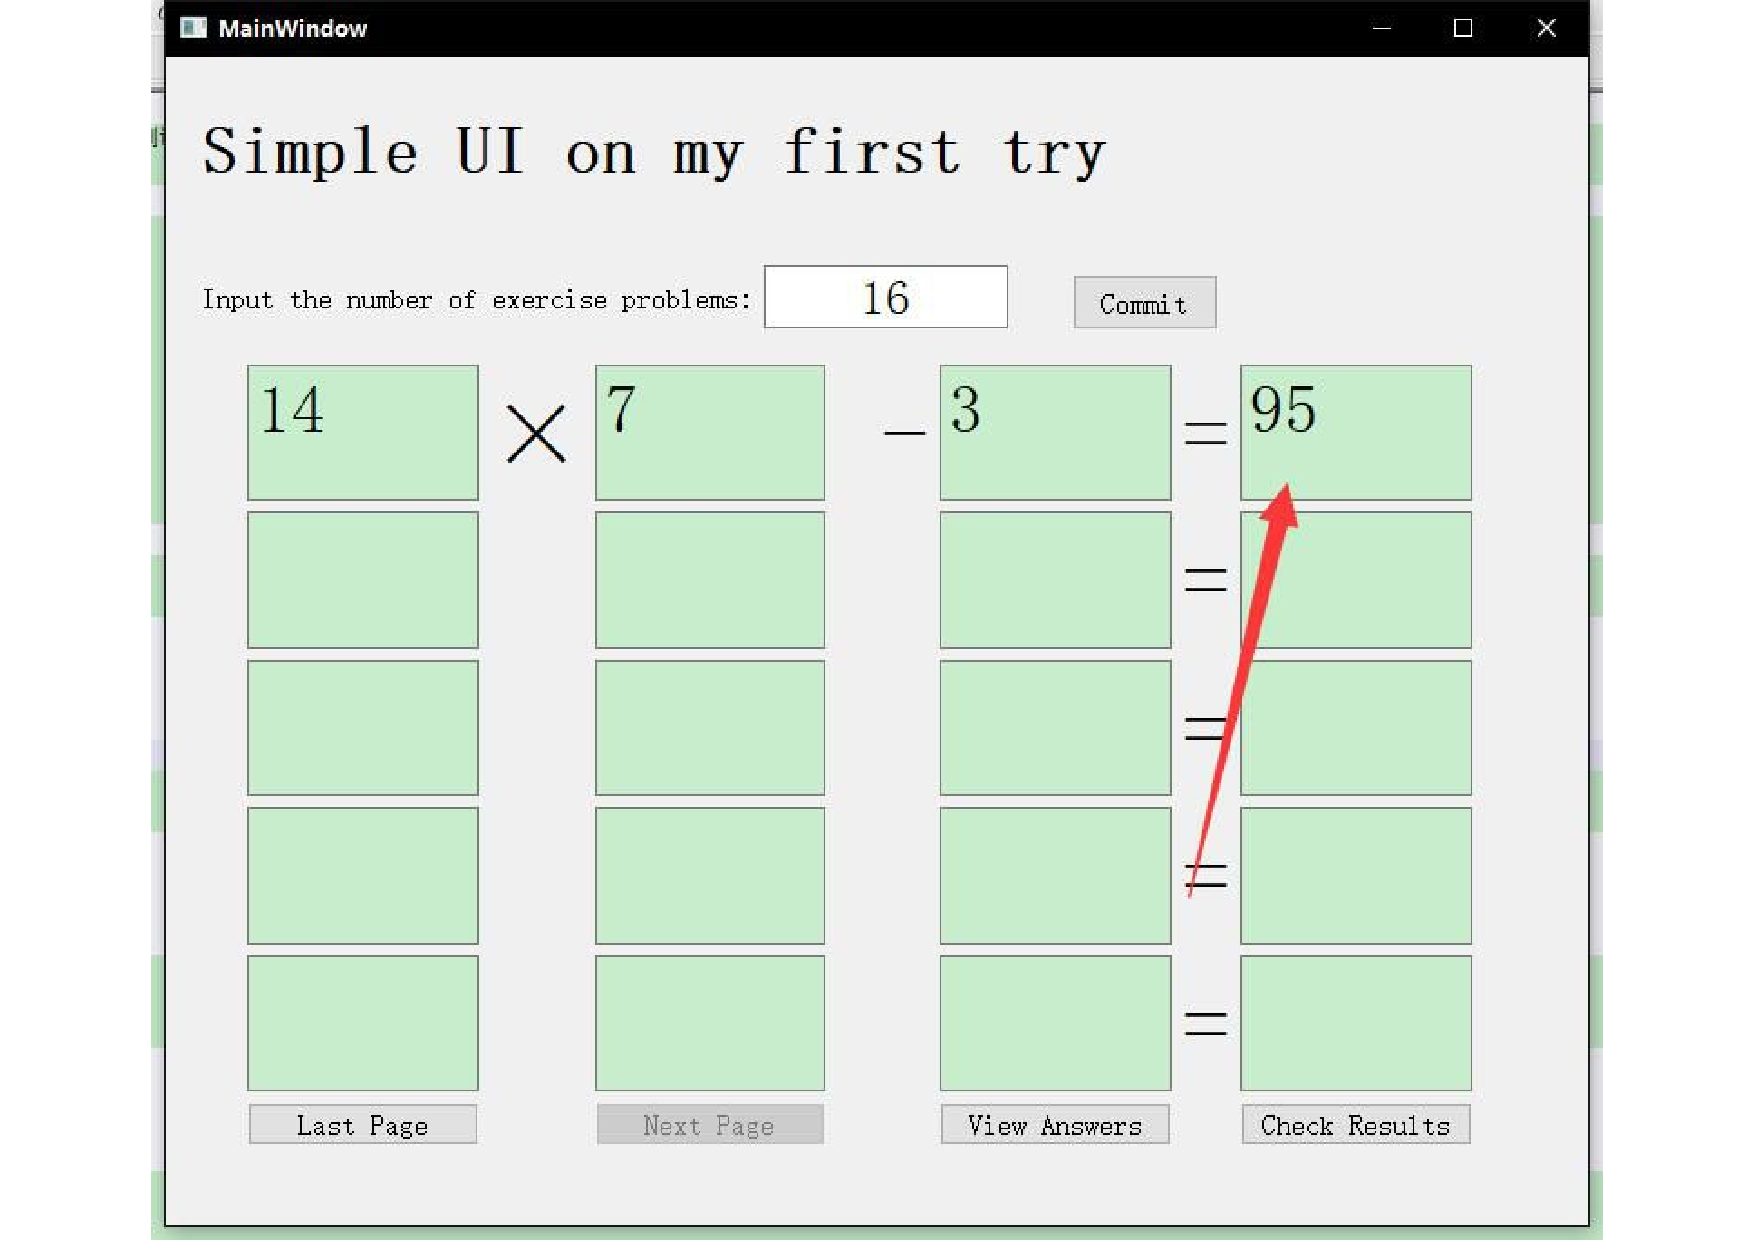
\includegraphics[width=2.5in]{./figures/9.pdf}
  \caption{Test 9}
  \label{Test_9}
\end{figure}

\end{CJK}
\end{document}
